\documentclass[10pt]{beamer}

\usetheme[progressbar=frametitle]{metropolis}
\usepackage{appendixnumberbeamer}

\usepackage{amsmath}
\usepackage{amssymb}
\usepackage{standalone}
\usepackage{hyperref}
\usepackage{cancel}

\usepackage{booktabs}
\usepackage[scale=2]{ccicons}
\usepackage{natbib}

\usepackage{pgfplots}
\usepgfplotslibrary{dateplot}

\setbeamercovered{transparent}

\usepackage{xspace}

% \newcommand{\bknote}[1]{{\color{cyan} BK: #1}}
\newcommand{\bknote}[1]{}

\newcommand{\hessian}{\mathcal{H}\xspace}


\graphicspath{{images/}}



\title{Security and Privacy of Machine Learning}
\date{July 2019}
\author{Bogdan Kulynych}

\begin{document}

\maketitle

% \begin{frame}{About Me}
%   \begin{itemize}
%     \item PhD student at EPFL, Switzerland
%     \item Previous lives: Kyiv-Mohyla Academy, Polytechnic University of Madrid, CERN, Google
%     \item Researching privacy and security and ML, counteracting harmful ML applications
%   \end{itemize}
% \end{frame}

% \begin{frame}{This class}
%   \begin{itemize}
%     \item Hopefully a lot of discussions in a group
%     \item Don't be afraid to say stupid things
%     \item Respect what others have to say, keep interruptions to a minimum
%   \end{itemize}
% \end{frame}

\begin{frame}{Table of contents}
  \setbeamertemplate{section in toc}[sections numbered]
  \tableofcontents[hideallsubsections]
\end{frame}

\section{Security and Privacy of ML?}

\begin{frame}[fragile]{The Holy Grail}
  \[
      \theta^* = \arg \min_\theta \mathbb{E}_{(x, y) \sim_{\alert{i.i.d.}} D} L(x, y; \theta)
  \]
\end{frame}

\begin{frame}[fragile]{}
  \begin{figure}
  \centering
  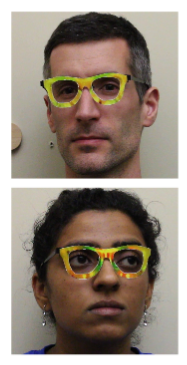
\includegraphics[width=1.5in]{glasses_intro.png} \\
  \footnotesize Image Credit: \cite{SharifBBR16}
  \end{figure}
\end{frame}

\begin{frame}[fragile]{}
  \begin{figure}
  \centering
  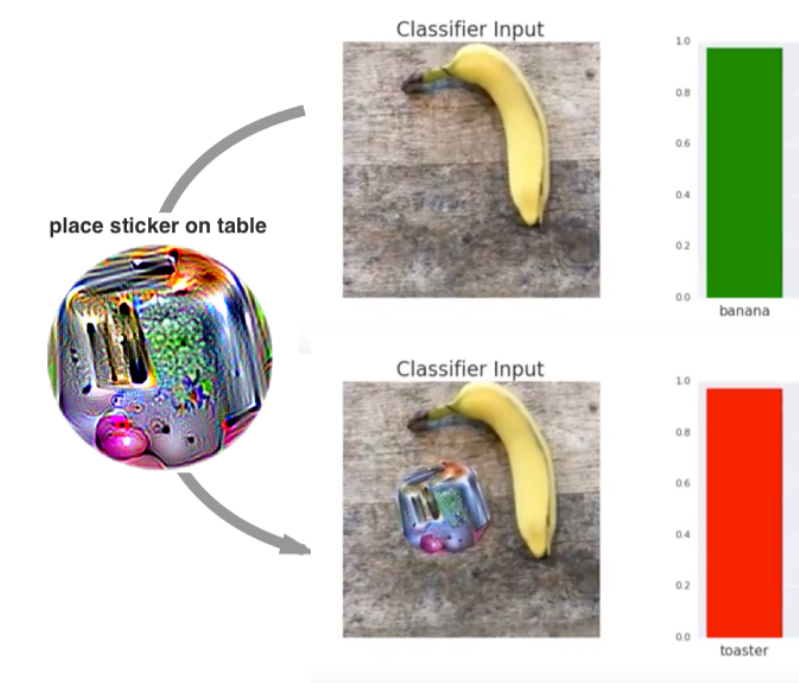
\includegraphics[width=3in]{patch.png} \\
  \footnotesize Image Credit: \cite{BrownMRAG17}
  \end{figure}
\end{frame}

\begin{frame}[fragile]{}
  \begin{figure}
  \centering
  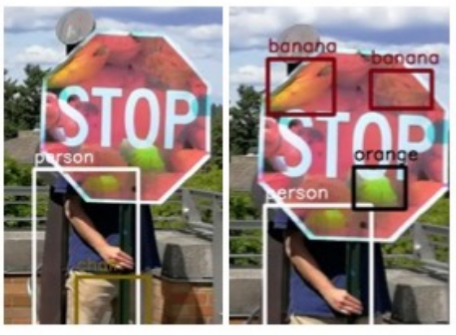
\includegraphics[width=3in]{patch_sign.png} \\
  \footnotesize Image Credit: \cite{SongEEF0RTPK18}
  \end{figure}
\end{frame}

\begin{frame}[fragile]{}
  \begin{figure}
  \centering
  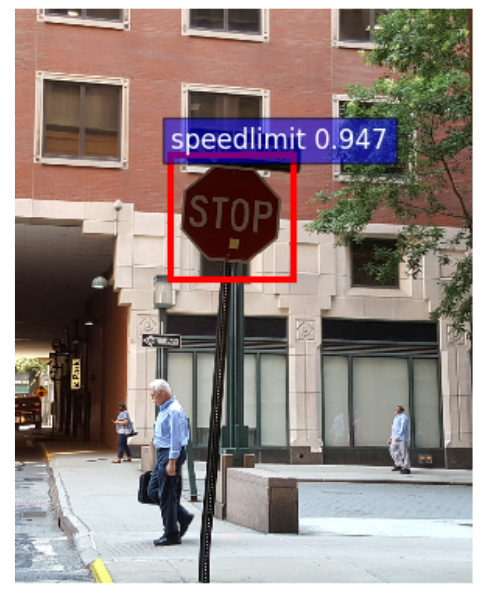
\includegraphics[width=2in]{backdoor.png} \\
  \footnotesize Image Credit: \cite{GuLDG19}
  \end{figure}
\end{frame}

\begin{frame}[fragile]{}
  \begin{figure}
  \centering
  
\includegraphics[width=3in]{echo_chamber.png} \\
  \end{figure}
\end{frame}

\begin{frame}[fragile]{}
  \begin{figure}
  \centering
  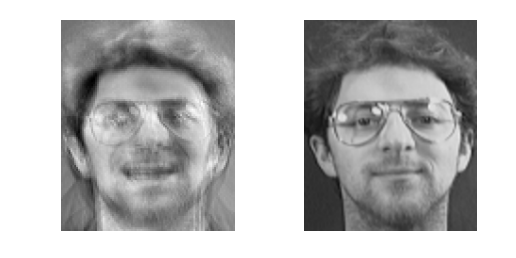
\includegraphics[width=3in]{inversion.png} \\
  \footnotesize Image Credit: \cite{FredriksonJR15}
  \end{figure}
\end{frame}

\begin{frame}[fragile]{}
  \begin{figure}
  \centering
  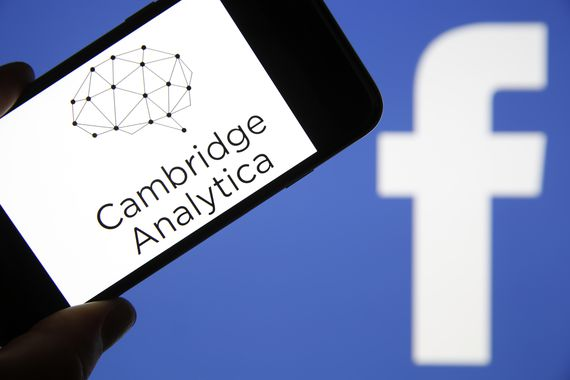
\includegraphics[width=3in]{cambridge_analytica.jpg} \\
  \end{figure}
\end{frame}


\section{Modern Security Principles}


\begin{frame}{Image Perturbations}
  \begin{figure}
    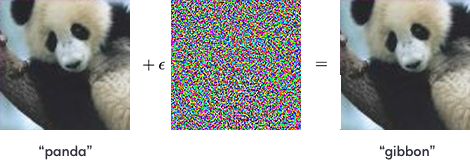
\includegraphics[width=2in]{panda.png} \\
    \footnotesize Image Credit: \cite{GoodfellowSS14}
  \end{figure}

  Imagine an algorithm $\textsf{Magic}(f, x, \tilde y) \mapsto \tilde x$:
  \begin{itemize}[<+-| alert@+>]
    \item Takes any computer vision classifier $f(x)$.
    \item Takes any image $x$ and target label $\tilde y$.
    \item Magically perturbs the image in an imperceptible way: $\tilde x$.
    \item Resulting image is missclassified by $f$ as anything you want ($\tilde y$).
  \end{itemize}

  % Groupwork.
  \visible<+->{
  \begin{alertblock}{Group discussion}
    Is this an attack?
  \end{alertblock}
}

\end{frame}

\begin{frame}{Context Matters}
    \begin{itemize}[<+-| alert@+>]
    \item Who performs the attack? What settings?
    \item What can the attacker do? What are the costs?
    \item What does the attacker know about the target?
    \item If the attack succeeds, why does it matter?
    \item In general: need \emph{context}.
    \item Many methodologies to formalize these.
  \end{itemize}
\end{frame}


\begin{frame}[fragile]{Generic High-Level Method: Threat Model}

  \begin{alertblock}{Threat Model}
  \begin{itemize}[<+-| alert@+>]
    \item \textbf{Threat:} \emph{What} are the bad things that can happen
      \begin{itemize}
        \item Spammers can get past your spam filter
      \end{itemize}
    \item \textbf{Risk:} \emph{How much} the exploitation of the threat will cost you
        \begin{itemize}
          \item People stop using your email service
        \end{itemize}
    \item \textbf{Attack:} \emph{How} can the threat be exploited
  \end{itemize}
  \end{alertblock}

  \begin{itemize}[<+->]
    \item This approach is useful for assessing risks, and prioritzing threats.
  \end{itemize}

\end{frame}


\begin{frame}[fragile]{Working Method: Adversary Model}

  \begin{alertblock}{Adversary Model}
  \begin{itemize}[<+-| alert@+>]
    \item ``Know the enemy and know yourself'' \\
          -- Sun Tzu, ``Art of War", 500 BC
    \item \textbf{Adversarial Goals}: What does the adversary \emph{want to achieve}
    \item \textbf{Adversarial Capabilities}: What does the adversary \emph{can do}
    \item \textbf{Adversarial Knowledge}: What does the \emph{adversary know} about you and your system
  \end{itemize}
  \end{alertblock}

  \begin{itemize}[<+-| alert@+>]
    \item More detailed than the previous model
    \item Enables comparisons of attacks, and principled approach to \emph{defenses}
    \item Phrase ``threat model'' and ``adversary model'' are often used interchangeably. Normally
        people mean ``adversary model''
    \item Impact (risks) of the attack is usually implicit, but we must keep them in mind.
  \end{itemize}
\end{frame}


\begin{frame}[fragile]{Adversary Model Example: Spam Email}
  \begin{itemize}[<+->]
    \item \textbf{Adversarial Goals}: Get an email past the spam detector.
    \item \textbf{Adversarial Capabilities}:
        \begin{itemize}
            \item Modify email content as long as some meaning is still preserved
            \item Send emails from different addresses
        \end{itemize}
    \item \textbf{Adversarial Knowledge}: Does not know how detector works, but observes if the
        email was classified as spam or not spam
  \end{itemize}
\end{frame}


\begin{frame}{Recall: Image Perturbations}
  \begin{figure}
    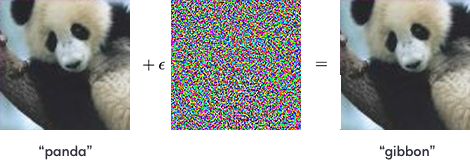
\includegraphics[width=2in]{panda.png} \\
    \footnotesize Image Credit: \cite{GoodfellowSS14}
  \end{figure}

  Imagine an algorithm $\textsf{Magic}(f, x, \tilde y) \mapsto \tilde x$:
  \begin{itemize}
    \item Takes a computer vision classifier and its parameters $f(x)$.
    \item Takes any image $x$ and target label $\tilde y$.
    \item Magically perturbs the image in an imperceptible way: $\tilde x$.
    \item Resulting image is missclassified by $f$ as anything you want ($\tilde y$).
  \end{itemize}

  % Groupwork.
  \begin{alertblock}{Group discussion:}
      \begin{itemize}[<+-| alert@+>]
          \item Who is the adversary? Who is the \emph{defender?}
          \item What are the possible settings and scenarios?
          \item What is the adversary model? What is the threat model?
      \end{itemize}
  \end{alertblock}

\end{frame}


\begin{frame}[fragile]{Adversary Model Example: Image Perturbations}
  \begin{description}[<+->]
    \item[Classifier] Instagram's detector of porn and nudity
    \item[Adversary] People that want to distribute porn on Instagram anyway
    \item[Threat] Users see nudes
    \item[Risk] This might breach laws and you get fined
    \item[Goals] Wants the detector to not detect
    \item[Capabilities] Modify the image as long as the semantics is preserved
    \item[Knowledge] Knows the exact classifier and its parameters
  \end{description}

\end{frame}


\begin{frame}{Defending Against the Attack}
  \begin{description}
    \item[Goals] Wants the detector to not detect the image
    \item[Capabilities] Modify the image as long as the semantics is preserved
    \item[Knowledge] Knows the exact classifier and its parameters
  \end{description}

  % Poll
  \pause
  \begin{alertblock}{Questions}
    \begin{enumerate}[<+->]
      \item Is this adversarial model realistic? Yes/No
      \item What is the best defense strategy?
        \begin{enumerate}
          \item Enforce strict access control inside Instagram to ensure model parameters cannot leak.
          \item Ensure that the \textsf{Magic} algorithm does not become publicly known. Use legal
            means (e.g., sue people or platforms that publicize it)
          \item Try to find kinds of classifiers that \textsf{Magic} algorithm does not work with.
        \end{enumerate}
    \end{enumerate}
  \end{alertblock}

\end{frame}


\begin{frame}[fragile]{Need to Attack in order to Defend}
  \begin{alertblock}{Principle}
    To defend, need to know how the adversary would attack.
  \end{alertblock}

  \pause
  \begin{itemize}[<+-| alert@+>]
    \item This is why adversary models are important
    \item Need to work on coming up with new attacks, and incentivize white-hat hackers to
      \emph{responsibly disclose} the attacks to you (e.g., via rewards).
  \end{itemize}
\end{frame}


\begin{frame}[fragile]{Worst-Case Security Principle}
  \begin{alertblock}{Principle}
    Do not underestimate your adversary. Strive to defend against the most powerful adversary, even
    if some aspects of the model might seem unrealistic.
  \end{alertblock}

  \pause
  \begin{itemize}[<+-| alert@+>]
    \item Kerckhoffs' Principle. As a defender, assume the attacker that \emph{knows} everything about your system.
    \item In general, more powerful attacker $\implies$ more knowledge, more capabilities.
    \item You should defend against an attacker that is as powerful as possible.
  \end{itemize}
\end{frame}


\begin{frame}[fragile]{Worst-Case Security Principle (flipped)}
  \begin{alertblock}{Principle}
    When designing an attack, strive to achieve most with the least power.
  \end{alertblock}

  \pause
  \begin{itemize}[<+-| alert@+>]
    \item A good attack means the attacker achieves the goals with as little capabilities and
      knowledge as possible.
  \end{itemize}
\end{frame}


\begin{frame}[fragile]{How to Defend?}
  \begin{description}
    \item[Goals] Wants the detector to not detect the image
    \item[Capabilities] Modify the image as long as the semantics is preserved
    \item[Knowledge] Knows the exact classifier and its parameters
  \end{description}

  % Poll
  \begin{alertblock}{Question}
    What is the best defense strategy?
  \end{alertblock}

    \begin{enumerate}
      \item Enforce strict access control inside Instagram to ensure model parameters cannot leak.
      \item Ensure that the \textsf{Magic} algorithm does not become publicly known. Use legal
        means (e.g., sue people or platforms that publicize it)
      \item Try to find kinds of classifiers that \textsf{Magic} algorithm does not work with.
    \end{enumerate}
\end{frame}


\begin{frame}[fragile]{How to Defend? (Answers)}
  \begin{enumerate}[<+-| alert@+>]
    \item Enforce strict access control inside Instagram to ensure model parameters cannot leak.
      \begin{enumerate}
        \item Worst-case security principle breached: \emph{Security by obscurity}
        \item What if they leak: get stolen or reverse engineered?
      \end{enumerate}
    \item Ensure that the \textsf{Magic} algorithm does not become publicly known. Use legal
      means (e.g., sue people or platforms that publicize it)
      \begin{enumerate}
        \item Worst-case security principle breached: \emph{Security by obscurity}
        \item Eventually the algorithm will be known: spread or sold.
        \item Know-the-attacks principle breached.
        \item Punishing researchers that find security vulnerability is a huge no-no.
          They need to be encouraged to disclose vulnerabilities to you, not punished.
      \end{enumerate}
    \item Try to find kinds of classifiers that \textsf{Magic} algorithm does not work with.
      \begin{enumerate}
        \item Worst-case adversary: knows the parameters of the model
      \end{enumerate}
  \end{enumerate}
\end{frame}


\begin{frame}[fragile]{Takeaways}
  \begin{itemize}[<+->]
    \item Know your adversary and know yourself: specify adversary's goals, capabilities, and
      knowledge.
    \item Need to find and encourage the discovery \emph{and responsible disclosure} of attacks --
      to fix them before they are exploited
    \item When defending, defend against even the strongest possible adversary model and attacks
    \item When attacking, try to achieve adversarial goals with the least power
  \end{itemize}
\end{frame}


\section{Adversary Models for Security and Privacy of ML}

\begin{frame}[fragile]{Machine Learning Pipeline}
  \includestandalone[width=\textwidth]{figs/mlthreat}
\end{frame}

\begin{frame}[fragile]{Adversary's Capabilities}
  \centering
  \includestandalone[width=3in]{figs/mlthreat}

  % Socratic
  \begin{alertblock}{Question}
    What could be the adversary's capabilities?
  \end{alertblock}

  \pause

  % TODO: Fix this list
  \begin{itemize}[<+-| alert@+>]
    \item Modify or supply new testing examples $x$
    \pause
    \item Modify or supply new training data $X$
    \pause
    \item Modify or supply new pre-trained components $g_{\theta'}$
    \pause
    \item Observe outputs (passive adversary)
  \end{itemize}
\end{frame}


\begin{frame}[fragile]{Adversary's Knowledge}
  \centering
  \includestandalone[width=3in]{figs/mlthreat}

  % Socratic
  \begin{alertblock}{Question}
    What could be the options for adversary's knowledge?
  \end{alertblock}

  \pause

  % TODO: Fix this list
  \begin{itemize}[<+-| alert@+>]
    \item No 100\% consistent terms
    \pause
    \item White-box: usually architecture $f$, parameters $\theta$, procedure $T$
    \pause
    \item Black-box: often knows architecture $f$ but no parameters, and has query access to $f$
        \emph{or} $T$
    \pause
    \item Agnostic black-box: only query access to $f$ \emph{or} $T$
  \end{itemize}

\end{frame}


\begin{frame}[fragile]{Adversary's Goals}
  \centering
  \includestandalone[width=3in]{figs/mlthreat}

  % Socratic
  \begin{alertblock}{Question}
    What could be adversary's goals?
  \end{alertblock}

  \pause

  % TODO: Fix this list
  \begin{itemize}[<+-| alert@+>]
    \item \emph{Evade the classifier} at test time: provide an \emph{adversarial example} $x$ that
      causes a mistake
    \pause
    \item Increase errors or make the classifier behave in a specific way
    \begin{itemize}
      \item by \emph{poisoning} the training data $X$
      \item by \emph{poisoning} the pre-trained model $g_{\theta'}$
    \end{itemize}
    \pause
    \item \emph{Steal} the model weights $\theta$
    \pause
    \item \emph{Infer} information about training data $X$.
  \end{itemize}

\end{frame}


\section{Active Attacks at Test Time}


\begin{frame}[fragile]{Evasion Attacks}
  \begin{figure}
    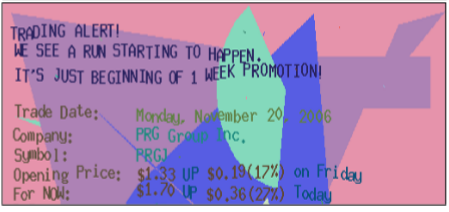
\includegraphics[width=2in]{spam.png} \\
    \footnotesize Image Credit: \cite{BiggioR18}
  \end{figure}

  \begin{itemize}[<+-| alert@+>]
    \item A goal of an \emph{evasion attack} is to evade detection, e.g., spam detection, fraud
      detection
    \item Goes back to 2004 in the context of Na\"ive Bayes spam classification (\cite{DalviDMSV04,
      LowdM05})
    \item Evasion attacks are done with \textbf{adversarial examples}:
      \begin{quote}
        Examples constructed by an adversary to deliberately cause a classification mistake
      \end{quote}
  \end{itemize}
\end{frame}


\begin{frame}[fragile]{Discovery of Non-Robustness of Neural Nets}

  \begin{figure}
    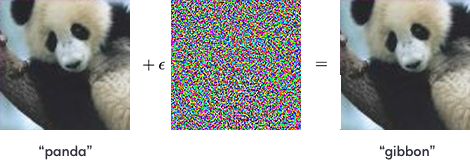
\includegraphics[width=2in]{panda.png} \\
    \footnotesize Image Credit: \cite{GoodfellowSS14}
  \end{figure}

  \begin{itemize}[<+->]
    \item \citet{SzegedyZSBEGF13} discover that outputs of neural nets are not robust to
      specially crafted imperceptible patterns. Authors pose it as a question of security.
    \item This attracted great interest in ML and Security communities with a long line of
      similar attack algorithms and defences
    \item Attacks work for any ML models, not only neural nets
    \item Because this line of work is very known, when people mention \emph{adversarial
      attacks}, \emph{adversarial robustness}, and \emph{adversarial examples} in ML, they usually
      talk about ``imperceptible perturbations that change classification outputs''
  \end{itemize}
\end{frame}


\begin{frame}{Image Perturbations}
  \begin{figure}
    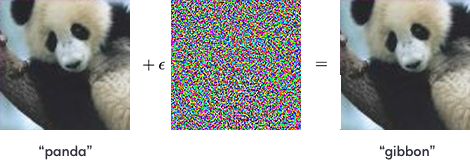
\includegraphics[width=2in]{panda.png} \\
    \footnotesize Image Credit: \cite{GoodfellowSS14}
  \end{figure}

  Can we build the image perturbation algorithm?
  \begin{itemize}[<+-| alert@+>]
    \item Goal: missclassify $x, y$ as something else
    \item Initial example $x, y$
    \item Perturbation $\delta$
    \item Perturbed image $x + \delta$
    \item Small perturbation:
      $\Delta = \{ \delta ~|~ \parallel \delta \parallel < \varepsilon \}$
    \item Model parameters $\theta$
    \item Loss of the model $L(x, y; \theta)$
  \end{itemize}

  % Groupwork.
  \visible<+->{
  \begin{alertblock}{Group discussion:}
    \bknote{TODO: Didn't work at all as a group discussion}
    How can we do it? What is the optimization problem?
  \end{alertblock}
  }
\end{frame}


\begin{frame}{Image Perturbations}

  \begin{columns}[T,onlytextwidth]

    \column{0.5\textwidth}
      \begin{alertblock}{Optimization problem}
        \[
          \begin{aligned}
            \delta^* =& \arg \max_{\delta} L(x + \delta, y; \theta) \\
            \text{ s.t. } & \parallel \delta \parallel \leq \varepsilon
          \end{aligned}
        \]
      \end{alertblock}

      % Socratic.
      \visible<+->{
      \begin{alertblock}{Question:}
        How do we solve it?
      \end{alertblock}
      }

    \column{0.5\textwidth}
      \includestandalone[width=2in, trim=0.0in 0.0in 0.0in 0.0in]{figs/advexopt}

  \end{columns}

\end{frame}


\begin{frame}{Gradient Descent}
  \begin{columns}[T,onlytextwidth]
    \column{0.5\textwidth}

    \begin{alertblock}{Optimization problem}
      \[
        \begin{aligned}
          \delta^* =& \arg \max_{\delta} L(x + \delta, y; \theta) \\
          \text{ s.t. } & \parallel \delta \parallel \leq \varepsilon
        \end{aligned}
      \]
    \end{alertblock}

    \begin{itemize}[<+-| alert@+>]
      \item Basic gradient descent (technically, ascent): \[
          \delta := \delta + \alpha \nabla_\delta L(x + \delta, y; \theta)
      \]
      \item How to meet the constraint?
    \end{itemize}

    \column{0.5\textwidth}
      \includestandalone[width=2in, trim=0.0in 0.0in 0.0in 0.0in]{figs/graddescent}

  \end{columns}

\end{frame}


\begin{frame}{Descent with Constraints}
  \begin{columns}[T,onlytextwidth]
    \column{0.5\textwidth}

    \begin{itemize}[<+-| @alert+>]
      \item Step, then project: \[
        \delta := \mathcal{P}_\Delta
          [ \delta + \alpha \nabla_\delta L(x + \delta, y)]
      \]
    \end{itemize}

    % Socratic
    \visible<+->{
    \begin{alertblock}{Question}
      For $x$ that were in training, $\nabla_x L(x, y; \theta)$ is small. What is the problem with
      small gradient values?
    \end{alertblock}
    }

    \column{0.5\textwidth}
      \begin{figure}
      \centering
      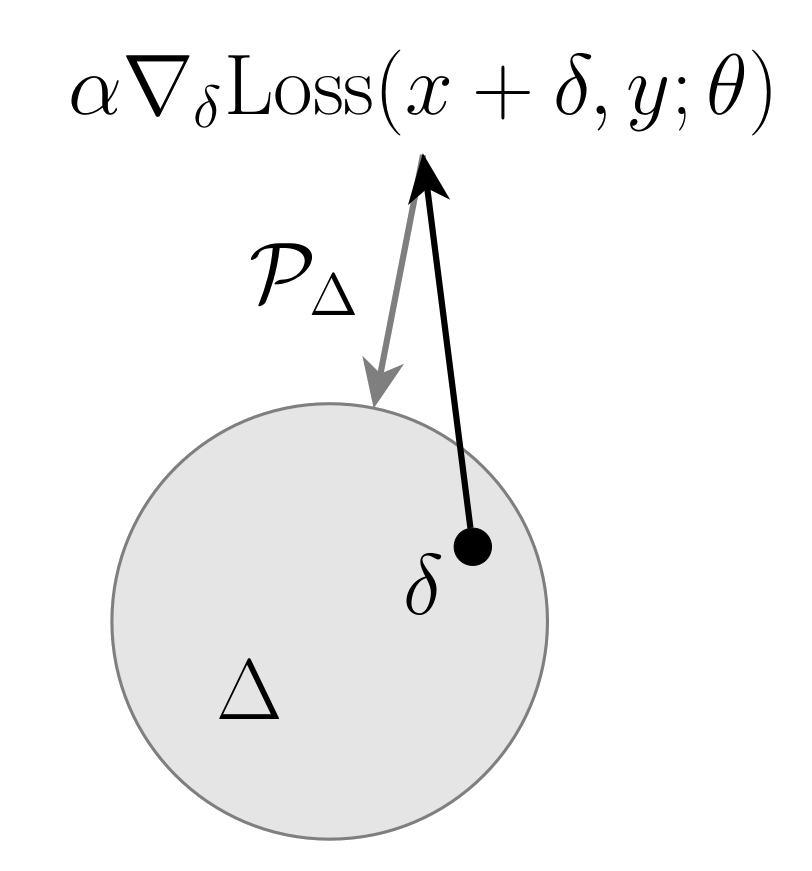
\includegraphics[width=1.5in]{projected_l2.png}
      \\
      {\footnotesize Image: Zico Kolter}
      \end{figure}

  \end{columns}

\end{frame}


\begin{frame}{Projected Gradient Descent (PGD)}

  \begin{itemize}[<+->]
    \item Final version proposed by \citet{MadryMSTV17}:
    \[
      \delta := \mathcal{P}_\Delta
        \left[ \delta + \alpha \ \alert{\textsf{sgn}}(\nabla_\delta L(x + \delta, y))\right]
    \]
    \item Run the algorithm for many (thousands of) steps until convergence
    \item Random restarts with different initial $\delta \in \Delta$
  \end{itemize}

\end{frame}


\begin{frame}{Projected Gradient Descent for $\ell_\infty$}
  \begin{columns}[T,onlytextwidth]

    \column{0.5\textwidth}
    % Socratic
    \begin{alertblock}{Question}
      Let $\Delta = \{ \delta ~|~ \parallel \delta \parallel_{\infty} \leq \varepsilon \}$.
      How do we project back to $\Delta$?
    \end{alertblock}

    \visible<+(1)->{
    \begin{itemize}[<+->]
      \item Projection:
        \[
          \mathcal{P}_\Delta(\delta) = \textsf{Clip}_\varepsilon[ \delta ] =
          (\max\{\delta_i, \varepsilon\})_i
        \]
      \item PGD update:
      \[
        \delta := \textsf{Clip}_\varepsilon
        \left[ \delta + \alpha \textsf{sgn} (\nabla_\delta L(x + \delta, y)) \right]
      \]
    \end{itemize}
    }

    \column{0.5\textwidth}
      \begin{figure}
      \centering
      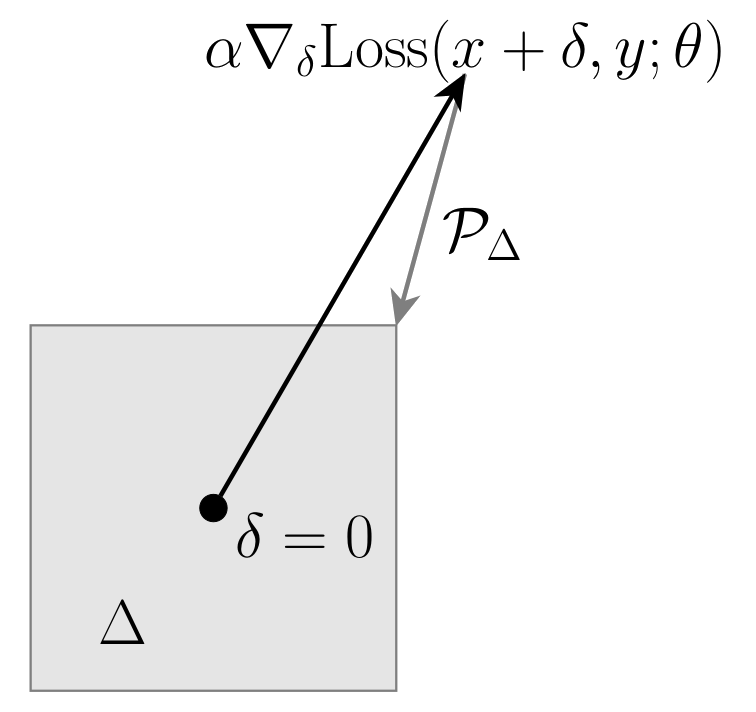
\includegraphics[width=1.5in]{projected_linf.png}
      \\
      {\footnotesize Image: Zico Kolter}
      \end{figure}

  \end{columns}
\end{frame}


\begin{frame}{Evasion Attacks with PGD}
  \begin{alertblock}{Group Discussion}
    What is the adversary model for an attack with PGD? Is this a powerful attacker?
  \end{alertblock}

  \visible<+(1)->{
  \begin{description}[<+-| @alert+>]
    \item[Goals] Cause a classification mistake
    \item[Capabilities] Adversary can construct modifications of existing examples of the following
      form:
      \[ \tilde{x} = x + \delta, \quad \parallel \delta \parallel \leq \varepsilon \]
      We assume this means ``imperceptible''.
    \item[Knowledge] White-box, need loss $L(\cdot)$ and parameters of the model $\theta$
  \end{description}
  }
\end{frame}


\begin{frame}{Properties of Adversarial Examples}
  \begin{itemize}[<+-| @alert+>]
    \item Let $\tilde x$ be an adversarial example for model $f_\theta(\cdot)$
    \item \textbf{Transferability:} It is likely to be missclassified by another model $f'$ trained on
      the same dataset
    \item \textbf{Black-box:} You can create a surrogate of the target model $f'$, and the
      adversarial example against $f'$ is likely to be missclassified by the actual target.
    \item \textbf{Resilience:} You can distort it (e.g., print) and it is likely to still be
      missclassified by $f_\theta$.
  \end{itemize}
\end{frame}


\begin{frame}{How to Defend?}
  \[
    \delta := \mathcal{P}_\Delta
      \left[ \delta + \alpha \ \textsf{sgn}(\nabla_\delta L(x + \delta, y))\right]
  \]

  \begin{alertblock}{Question}
    What is the best strategy to defend against adversarial examples like these?
  \end{alertblock}

  \begin{enumerate}[<+->]
    \item Ensure that the attacker cannot obtain parameters of the model $\theta$ through careful
      access controls.
    \item Ensure that all or overwhelming majority of examples $x \in \Delta$ are classified
      the same.
    \item During training, simulate the adversary and penalize its wins. In other words, generate
      adversarial examples and train on them with correct labels.
    \item Train the model in such a way that the gradient does not point in the best direction
    \item Preprocess the inputs to ensure small perturbations are blurred
  \end{enumerate}

\end{frame}


\begin{frame}{How to Defend? (Answers)}
  \begin{itemize}[<+->]
    \item Ensure that the attacker cannot obtain parameters of the model $\theta$ through careful
      access controls.
      \begin{itemize}
        \item Worst-case security principle breached: \emph{Security by obscurity}
      \end{itemize}

    \item Preprocess the inputs to ensure small perturbations are blurred
      \begin{itemize}
        \item Relies on the fact that the adversary does not know what is the preprocessing
        \item If adversary knew what was the preprocessing, they could adapt adversarial examples
          accordingly
        \item Hence, worst-case security principle breached: \emph{Security by obscurity}
      \end{itemize}

    \item Train the model in such a way that the gradient does not point in the best direction
      \begin{itemize}
        \item This is similar to \emph{Security by obscurity}
        \item There are other attacks that do not rely on the gradient.
      \end{itemize}
  \end{itemize}

\end{frame}


\begin{frame}{How to Defend? (Answers)}
  \begin{itemize}[<+->]
    \item Ensure that all or overwhelming majority of examples $x \in \Delta$ are classified
      the same.
      \begin{itemize}
        \item This is the ideal case.
        \item Impossible in practice, but this is what people strive for.
      \end{itemize}

    \item During training, simulate the adversary and penalize its wins. In other words, generate
      adversarial examples and train on them with correct labels.
      \begin{itemize}
        \item This is called \emph{adversarial training}
        \item In practice, this defence only approximately protects against a particular
          attack, but it works.
        \item This is your best bet at defending.
      \end{itemize}

  \end{itemize}

\end{frame}


\begin{frame}{Adversarial Training}
  \begin{itemize}[<+-| @alert+>]
    \item Regular loss minimization objective:
      \[
        \theta^* = \arg \min_\theta \sum_{x, y \in X} L(x, y; \theta)
      \]
    \item Recall: When defending, defend against even the strongest possible adversary model and
      attacks
    \item Adversarial loss minimization objective:
      \[
        \theta^* = \arg \min_\theta \sum_{x, y \in X} \underbrace{\max_{\delta \in \Delta}
        L(x + \delta, y; \theta)}_{\text{Adversarial example}}
      \]
    \item Best we can do: solve the inner maximization exactly. Even this does not guarantee that
        there exist no adversarial examples in $\Delta$
    \item PGD solves the inner maximization approximately $\implies$ approximate security, but works
      better than most other proposed defenses in practice
    \item In fact, instead of finding adversarial examples, you can just randomly sample many
      examples from $\Delta$ (\cite{CohenRK19})
  \end{itemize}
\end{frame}


\begin{frame}{Big Picture: Security Implications of Non-Robust Features}
  \begin{itemize}[<+-| @alert+>]
    \item Recent research suggests: ML is not robust to imperceptible
      perturbations, because models pick up \emph{non-robust features} specific to the dataset, that
      are not interpretable by humans (\cite{IlyasSTETM19})
    \item We have some idea on how to reduce the impact of this problem in $\Delta = \{ \delta ~|~
      \parallel \delta \parallel \leq \varepsilon \}$
  \end{itemize}

  \visible<+(1)->{
  \begin{alertblock}{Question}
      \bknote{TODO: This Socratic failed, no ideas pulled at all}
      Do the defenses before (fixing non-robust features) solve the security of ML against evasion attacks?
  \end{alertblock}

  \pause

  \begin{itemize}[<+-| @alert+>]
    \item The threat model of $\{ \delta ~|~ \parallel \delta \parallel \leq \varepsilon
      \}$ covers only one kind of attack.
    \item Opinion: ML community focuses on this adversarial robustness because of the mathematically
      elegent form
    \item Opinion: Robustness to imperceptible perturbations is more important to ML theory than
  ML security
  }

  \end{itemize}

\end{frame}


\begin{frame}{Beyond Imperceptible Perturbations}
  \begin{figure}
    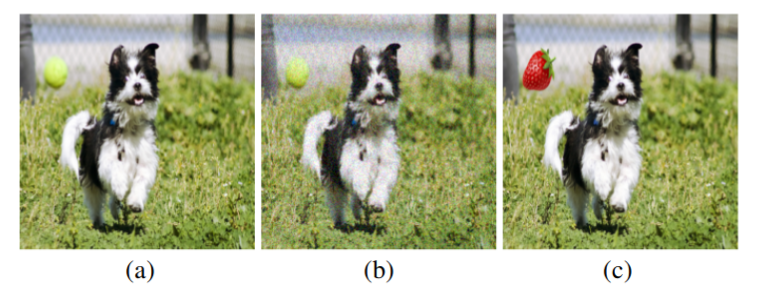
\includegraphics[width=3in]{dog.png} \\
    (b) and (c) have the same $\parallel \delta \parallel$ \\
    Image Credit: \cite{JacobsenBCTP19}
  \end{figure}
\end{frame}


\begin{frame}{Beyond Imperceptible Perturbations}
  \begin{figure}
    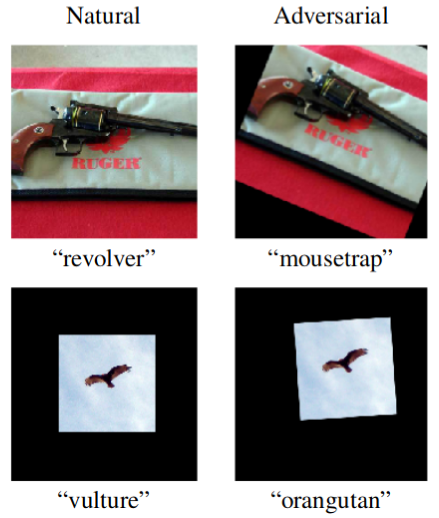
\includegraphics[width=2.1in]{rotation.png} \\
    Image Credit: \cite{EngstromTSM17}
  \end{figure}
\end{frame}


\begin{frame}{Beyond Imperceptible Perturbations}
  \begin{figure}
    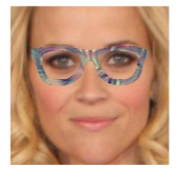
\includegraphics[width=2in]{glasses.png} \\
    These are not even imperceptible! \\
    Image Credit: \cite{SharifBBR16}
  \end{figure}
\end{frame}


\begin{frame}{Beyond Imperceptible Perturbations}
  \begin{figure}
    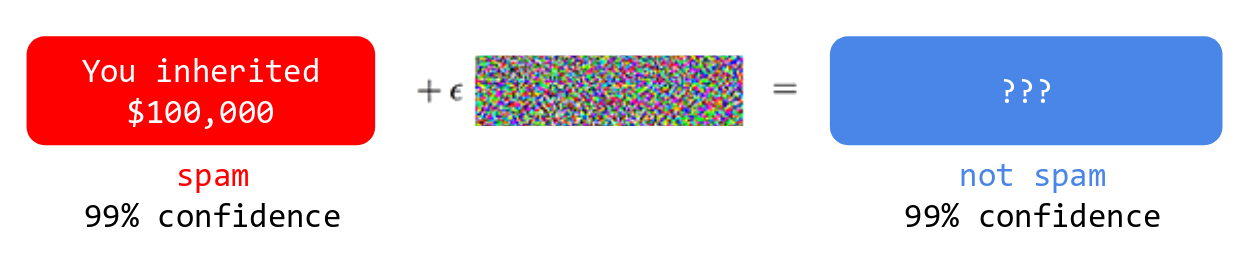
\includegraphics[width=3in]{discrete.png} \\
    What about discrete domains? \\
    See \cite{KulynychHST18}
  \end{figure}
\end{frame}


\begin{frame}{Takeaways}
  \begin{itemize}[<+-| @alert+>]
    \item Currently, discussion about adversarial robustness of ML at test time puts robustness to
      imperceptible perturbations in the spotlight
    \item This problem is of interest both to ML Theory and ML Security
    \item However, this likely is not the main security concern for your application, unless you
        have a security-critical image classifier
    \item There are many other attack vectors against classifiers at test time
    \item Beyond imperceptible perturbation for images, the field seems very much in its infancy,
      many open problems.
    \item Adversarial training approach likely provides some remedy from different kind of attacks --
      but without any formal guarantees
  \end{itemize}
\end{frame}


\begin{frame}{Quick Recap: Security Principles}

  \alert{Are any security principles violated here?}
  \begin{itemize}[<+-| @alert+>]
    \item You use a custom random-forest-based network-intrusion detection system (not open-source).
        You are not afraid of hackers evading it because they don't know how it works.
    \item A researcher has emailed you about a vulnerability in the computer vision system of your
        automated drones. You sue them.
    \item Your traffic-sign recognition system is provably robust to $\varepsilon=0.65$
        $\ell_1$-perturbations of all examples in your training set. This is state-of-the-art
        $\varepsilon$ for this task.
    \item You have went through all existing evasion attacks and have constructed a detector for each.
      It works 100\% of the time. In deployment, your model first runs the detector, and rejects
      the input if it looks like an adversarial example.
  \end{itemize}

\end{frame}


\section{Dealing with Black Boxes}


\begin{frame}{Recall: Adversarial Knowledge}

  \begin{itemize}[<+-| @alert+>]
    \item No 100\% consistent terms
    \item White-box: usually architecture $f$, parameters $\theta$, procedure $T$
    \item Black-box: often knows architecture $f$ but no parameters, and has query access to $f$
        \emph{or} $T$
    \item Agnostic black-box: only query access to $f$ \emph{or} $T$
  \end{itemize}

\end{frame}


\begin{frame}{Black-Box Access}

  \begin{itemize}[<+-| @alert+>]
    \item The PGD attack only works in the white-box setting: need the gradient $\nabla L$:
    \[
      \delta := \mathcal{P}_\Delta
        \left[ \delta + \alpha \ \textsf{sgn}(\nabla_\delta L(x + \delta, y))\right]
    \]
  \end{itemize}

  \visible<+->{
  \begin{alertblock}{Group Discussion}
    Can you attack if a model has non-differentiable components?
  \end{alertblock}
  }

  \visible<+->{
  \begin{alertblock}{Group Discussion}
    Can you attack if you only have query access to $f(\cdot)$?
  \end{alertblock}
  }

\end{frame}


\begin{frame}{Black-Box Attacks at Test Time}

  Classical approach (\cite{LowdM05})

  \pause
  \begin{enumerate}[<+-| @alert+>]
    \item Reverse engineer the model
    \item Run a white-box attack
  \end{enumerate}

  Smarter approach (\cite{ChenZSYH17})

  \begin{enumerate}[<+-| @alert+>]
    \item Run a black-box optimization algorithm that only needs query access to $f(\cdot)$
  \end{enumerate}

\end{frame}


\begin{frame}{Estimating the Gradient}

  \begin{itemize}[<+-| @alert+>]
    \item Can estimate the gradient in a black-box manner from two evaluations:
      \[
        \frac{d}{dx_i} f(x) = \frac{f(x + \delta e_i) - f(x - \delta e_i)}{2\delta}
      \]
      for small $\delta$, and basis vectors $e_i$.
    \item Attack principle: run PGD but estimate gradient in every iteration (\cite{ChenZSYH17})
  \end{itemize}

  \pause

  \visible<+->{
  \begin{alertblock}{You already know this from worst-case security but...}
    Adding non-differentiable components is not a valid defense.
  \end{alertblock}
  }

\end{frame}


\begin{frame}{Model Stealing}

  \begin{itemize}[<+-| @alert+>]
    \item We can also steal the model parameters by querying it many times
    \item Construct a large dataset $X' = \{(x, f(x)), ...\}$
    \item Train $f_{\theta'}$.
  \end{itemize}

  \pause

  \visible<+->{
  \begin{alertblock}{Question}
    Let $f(x)$ be a linear model. Its decision boundary is $h(x) = w \cdot x + b$.
    $w$~is a $750$-dimensional vector. How many queries are needed to steal $f(x)$?
  \end{alertblock}
  }

  \pause
  \begin{itemize}[<+-| @alert+>]
    \item Need $d + 1$ to steal a linear model using equation solving
    \item But, need a lot more queries to steal a neural net
    \item For a net with 2K parameters, need 11K queries to get 99.9\% similarity (\cite{TramerZJRR16})
  \end{itemize}

\end{frame}


\begin{frame}{Takeaways}

  \begin{itemize}[<+->]
    \item If your system is queriable by adversaries, it can be reverse-engineered (model stealing)
    \item Evasion attacks can be mounted even without reverse engineering: black-box attacks.
    \item
      You don't need the gradient to attack: non-differentiable classifiers can be attacked using
      black-box attacks
  \end{itemize}

\end{frame}


\section{Attacks at Training Time}


\begin{frame}[fragile]{Recall: Machine Learning Pipeline}
  \includestandalone[width=\textwidth]{figs/mlthreat}
\end{frame}


\begin{frame}[fragile]{Poisoning Attacks}
  \centering
  \includestandalone[width=2in]{figs/mlthreat}

  \begin{itemize}[<+-| alert@+>]
    \item Adversarial Goals: Reduce performance of the model or modify the task
    \item Adversarial Capabilities: Inject or modify training examples $X$, or pre-trained components
      $g_{\theta'}$
    \item Adversarial Knowledge: Knows the algorithm $T$
  \end{itemize}

  \begin{alertblock}{Question}
    Is this a realistic adversary model? Are there any relevant settings?
  \end{alertblock}
\end{frame}


\begin{frame}[fragile]{Poisoning Attacks with Poisoned Examples}
  Na\"ive approach:
  \begin{itemize}[<+-| alert@+>]
    \item Mess up with data (e.g., modify labels)
    \item Retrain and check if helped
    \item Adapt and repeat
  \end{itemize}

  \pause

  \begin{itemize}[<+-| alert@+>]
    \item Does not scale
    \item Retraining is a bottleneck
    \item Need a tool to guide what features or examples are important
  \end{itemize}

\end{frame}


\begin{frame}[fragile]{In Search of a Closed-Form Expression}

  \begin{itemize}[<+-| alert@+>]
    \item Recall the empirical loss minimization problem:
      \[
        \theta^* = \arg \min_\theta \sum_{x, y \in X} L(x, y; \theta)
      \]
    \item What if an example $z = (x, y)$ was upweighted by $\varepsilon$?
      \[
        \theta^*_{z, \varepsilon} = \arg \min_\theta \left[\sum_{x', y' \in X} L(x', y'; \theta) +
        \varepsilon L(z; \theta)\right]
      \]
    \item These correspond to two different classifiers
    \item Let's call the difference between their weights $\Delta$:
      \[
        \Delta_{z, \varepsilon} := \theta^*_{z, \varepsilon} - \theta^*
      \]
  \end{itemize}

\end{frame}


\begin{frame}[fragile]{Strategy: First-Order Approximation}

  \begin{enumerate}[<+-| alert@+>]
    \item Recall the first-order Taylor approximation:
      \[
        f(\mathbf{x}) \approx f(\mathbf{x}') + \nabla f(\mathbf{x}') \cdot (\mathbf{x} - \mathbf{x'})
      \]
    \item Recall the classifier with upweighted $z$:
      \[
        \theta^*_{z, \varepsilon} = \arg \min_\theta \underbrace{\sum_{x', y' \in X} L(x', y';
        \theta)}_{R(\theta)} + \varepsilon L(z; \theta)
      \]
    \item Recall that a global optimizer $\theta^*_{z, \varepsilon}$ satisfies:
      \[
        \nabla R(\theta^*_{z, \varepsilon}) + \varepsilon \nabla L(z; \theta^*_{\varepsilon, z}) = 0
      \]
  \end{enumerate}

  \pause
  \begin{alertblock}{Derivation}
    How can we get a first-order approximation of
      $\frac{d}{d\varepsilon} \Delta_{z, \varepsilon} = \frac{d}{d\varepsilon} [\theta^*_{z,
      \varepsilon} - \theta^*]$?
  \end{alertblock}

\end{frame}


\begin{frame}[fragile]{Deriving the Influence Function}

  \begin{enumerate}[<+-| alert@+>]
    \item Rewrite (3) in terms of $\theta^*$:
      \[
        \begin{aligned}
          0 \approx & [\nabla R(\theta^*) + \varepsilon \nabla L(z; \theta^*] + \\
          & [\hessian R(\theta^*) + \varepsilon \hessian L(z; \theta^*)]\ \Delta_{z, \varepsilon},
        \end{aligned}
      \]
      where $\hessian f(x)$ is a Hessian matrix.
    \item Solve for $\Delta_{z, \varepsilon}$:
      \[
        \begin{aligned}
          \Delta_{z, \varepsilon} \approx -[\nabla R(\theta^*) + \varepsilon \nabla L(z; \theta^*)] \\
            [\hessian R(\theta^*) + \varepsilon \hessian L(z; \theta^*)]^{-1}
        \end{aligned}
      \]
    \item Because $\nabla R(\theta^*) = 0$ and assuming $\varepsilon$ is small (\cite{KohL17}):
      \[
        \begin{aligned}
          \Delta_{z, \varepsilon} \approx -\varepsilon \nabla L(z; \theta^*) [\hessian R(\theta^*)]^{-1}
        \end{aligned}
      \]
  \end{enumerate}

\end{frame}


\begin{frame}[fragile]{Influence Function}

  \begin{enumerate}[<+-| alert@+>]
    \item We call the rate of change of $\Delta_{z, \varepsilon}$ \emph{the influence function}:
      \[
        \frac{d}{d\varepsilon} \Delta_{z, \varepsilon} = \nabla L(z; \theta^*) [\hessian R(\theta^*)]^{-1}
      \]
    \item What about poisoning examples? Let $z_\delta = (x + \delta, y)$
    \item Modify the upweighted model:
      \[
        \theta^*_{z, z_\delta, \varepsilon} = \arg \min_{\theta} [R(\theta) - \varepsilon L(z, \theta) +
        \varepsilon L(z_\delta, \theta)]
      \]
  \end{enumerate}

  \pause

  \visible<+->{
  \begin{alertblock}{Derivation}
    What is the expression for $\frac{d}{d\varepsilon} \Delta_{z, z_\delta, \varepsilon} =
     \frac{d}{d\varepsilon} \left[\theta^*_{z, z_\delta, \varepsilon} - \theta^* \right]$?
  \end{alertblock}
  }

\end{frame}


\begin{frame}[fragile]{Influence Functions for Poisoning}
  \begin{enumerate}[<+-| alert@+>]
    \item Same strategy as before:
      \[
        \begin{aligned}
          \Delta_{z, z_\delta, \varepsilon} \approx & [\nabla \cancel{R(\theta^*)} + \varepsilon \nabla L(z_\delta; \theta^*) - \varepsilon
          \nabla L(z; \theta^*)] + \\
          & [\hessian R(\theta^*) + \cancel{\varepsilon \hessian L(z; \theta^*) - \varepsilon
          \hessian L(z; \theta^*)}]^{-1}
        \end{aligned}
      \]
    \item You can see that:
      \[
        \frac{d}{d\varepsilon} \Delta_{z, z_\delta, \varepsilon} = \left[\frac{d}{d\varepsilon}
        \Delta_{z_\delta, \varepsilon} - \frac{d}{d\varepsilon} \Delta_{z, \varepsilon}\right]
      \]
    \item Final step: Influence on some target example $t$:
      \[
        \nabla \frac{d}{d\varepsilon} L(t; \theta^*_{z, z_\delta, \varepsilon}) \approx
        \nabla L(t; \theta^*) \cdot \frac{d}{d\varepsilon} \Delta_{z, z_\delta, \varepsilon}
      \]

  \end{enumerate}

  \pause
  \visible<+->{
  \begin{alertblock}{Question}
    How do we use this to build a poisoning attack to force a model to make a mistake on $t$?
  \end{alertblock}
  }

\end{frame}


\begin{frame}[fragile]{Influence Functions for Poisoning}
  \begin{itemize}[<+-| alert@+>]
    \item Reparameterize:
      \[
        Q(x, \delta; \theta) = L(t; \theta^*) \cdot \frac{d}{d\varepsilon} \Delta_{z, z_\delta, \varepsilon}
      \]
    \item Poisoning optimization problem:
      \[
        \delta^* = \arg \max_\delta Q(x, \delta; \theta) \text{ s.t. } \parallel \delta \parallel
        \leq \epsilon
      \]
    \item How to solve it?
    \pause
    \item PGD for poisoning:
      \[
        \delta := \mathcal{P}[\delta + \alpha \nabla_\delta Q(x, \delta; \theta)]
      \]
  \end{itemize}
\end{frame}


\begin{frame}{Poisoning Models}
  \begin{figure}
    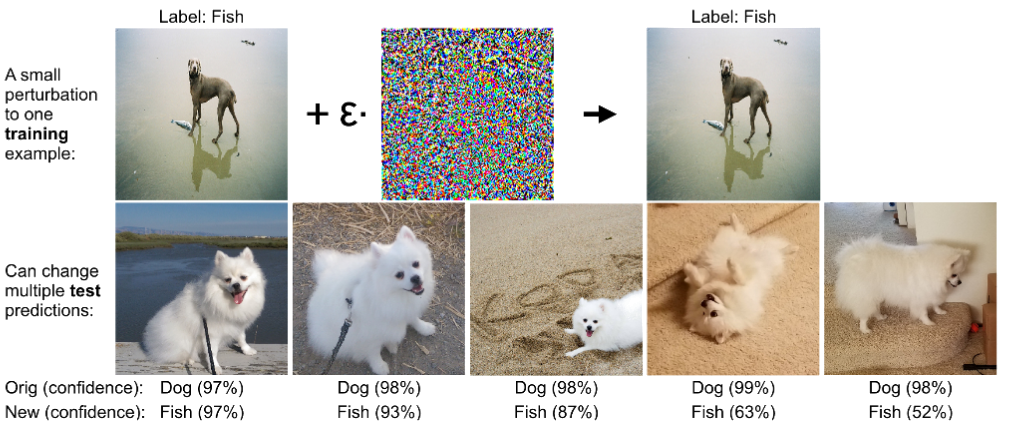
\includegraphics[width=4in]{poisoning_dog.png} \\
    Image Credit: \cite{KohL17}
  \end{figure}
\end{frame}


\begin{frame}{Many Settings of Poisoning}
  Possible goals:
  \begin{itemize}[<+-| alert@+>]
    \item Increase error
    \item Prevent convergence
    \item Increase error only on certain inputs (backdooring)
    \item Replace the model with the model of your choosing
    \item Modify a property of the model (e.g., fairness)
    \item Increase error
  \end{itemize}
  \begin{itemize}[<+-| alert@+>]
    \item Not discussing poisoning pre-trained models, but it is doable (\cite{BagdasaryanVHES18})
    \item There is hope for defences, but it is not developed well yet (\cite{SteinhardtKL17})
  \end{itemize}
\end{frame}

\begin{frame}[fragile]{Takeaways}
  \begin{figure}
    
\includegraphics[width=3in]{echo_chamber.png}
  \end{figure}
\end{frame}


\begin{frame}[fragile]{Takeaways}
  \begin{itemize}[<+-| alert@+>]
    \item Whenever the data is not trusted (e.g., federated learning), the trained model can be
      manipulated
    \item Adversaries might be able to modify the behaviour of models even if injecting a single example
    \item Universal defences are not there yet
  \end{itemize}
\end{frame}


\section{Privacy and Machine Learning}


\begin{frame}{Wait, what is privacy?}
  \begin{figure}
    \centering
    
\includegraphics[width=2.5in]{google_photos.png}
  \end{figure}
  \begin{alertblock}{Group discussion}
    What is happening here?
  \end{alertblock}
\end{frame}


\begin{frame}{Concepts of Privacy (One of Many Approaches)}
  \begin{itemize}[<+-| alert@+>]
    \item Institutional privacy
    \begin{itemize}
      \item Your data is private because Google promises so in their Privacy Policy
      \item Need to \textbf{trust Google}
    \end{itemize}
    \item Social privacy
    \begin{itemize}
      \item Your data is private because Google gives you fine-grained controls on when to share
        what photos and with whom
      \item Need to \textbf{trust Google}
    \end{itemize}
    \item Hard privacy (``surveillance privacy'')
    \begin{itemize}
      \item Your data is private because Google \emph{provably cannot see and access any of it}
      \item Often enforced through \emph{cryptography} and privacy-enhancing technologies
      \item Ideally need to \textbf{trust Math}
    \end{itemize}
    \item Privacy here will mean \emph{hard privacy}, not access controls or privacy policies
    \item \alert{Question:} What was happening with Google Photos?
  \end{itemize}
\end{frame}


\begin{frame}{Leaky Models}
  \begin{figure}
    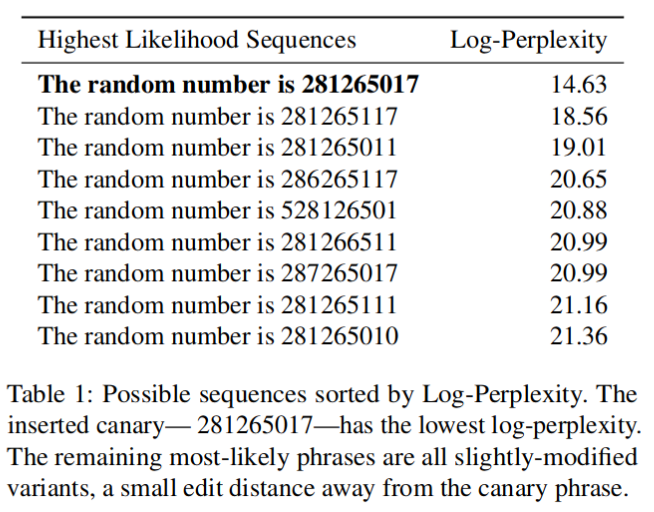
\includegraphics[width=2.8in]{secret_sharer.png}
  \end{figure}
  \begin{itemize}[<+-| alert@+>]
    \item High-capacity ML models memorize data (\cite{CarliniLKES18})
    \item Models behave differently on examples that were in training and that were not
  \end{itemize}
\end{frame}


\begin{frame}{The Goals of the Privacy Adversary}
  \begin{alertblock}{Question}
    What are the possible goals of the privacy adversary?
  \end{alertblock}

  \begin{itemize}[<+-| alert@+>]
    \item \textbf{Membership Inference:} Learn if an example $x$ was in the training dataset $X$ or not
    \item \textbf{Attribute Inference:} Knowing a part of an example $\tilde x$, learn the other part
    \item \textbf{Model Inversion:} Given a model, extract training data points
  \end{itemize}

  \pause

  \visible<+->{
  \begin{alertblock}{Question}
    Assuming one attribute is unknown, and it takes two different values (e.g., HIV status), how to
    mount an attribute inference attack using a membership inference attack?
  \end{alertblock}
  }
\end{frame}


\begin{frame}{Membership Inference}
  \begin{alertblock}{Question}
    What should be the capabilities of the adversary to perform membership inference?
  \end{alertblock}

  \pause
    \visible<+->{Surprisingly, agnostic black-box might be enough}
\end{frame}


\begin{frame}{Ad-Hoc: Confidence Distributions}
  \begin{figure}
    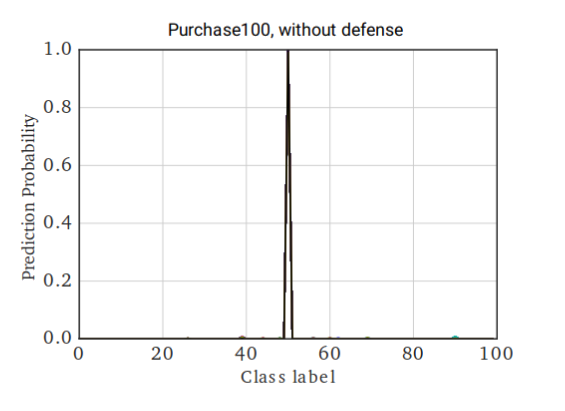
\includegraphics[width=3in]{confidences.png} \\
    Image Credit: \cite{NasrSH18}
  \end{figure}
\end{frame}


\begin{frame}{Shadow Model Attack}

  \begin{figure}
    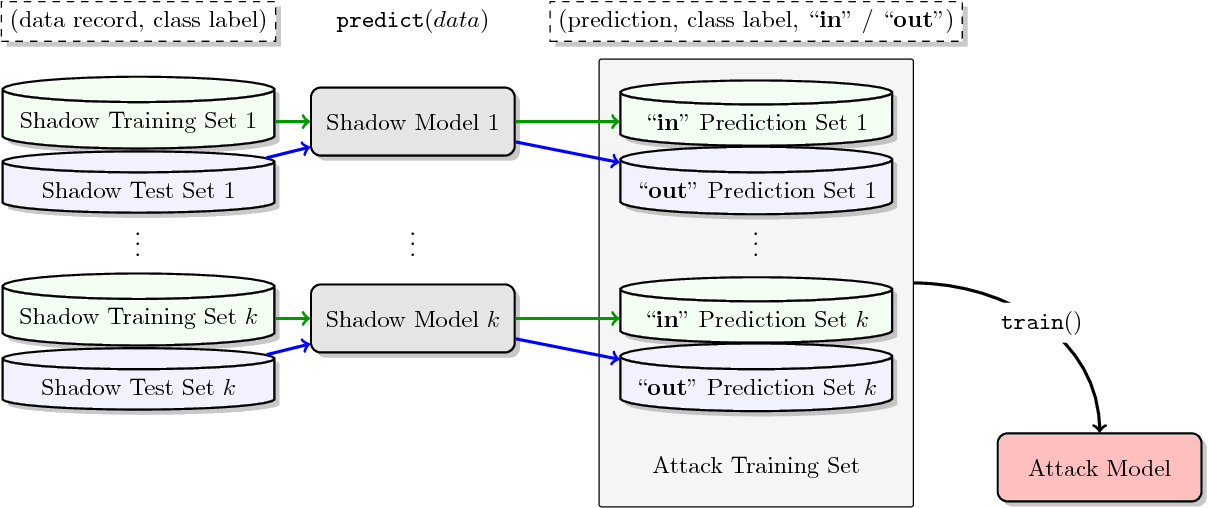
\includegraphics[width=2.8in]{shadows.png} \\
  \end{figure}

  \begin{itemize}[<+-| alert@+>]
    \item Pioneering membership inference attack (\cite{ShokriSS16})
    \item Adversary's knowledge: dataset $X_A$ coming from the same distribution as $X$, model
        architecture $f$, query access to $f_{\theta}$
    \item Adversary's goal: learn if $x$ was in training $X$
    \item Train a bunch of \emph{shadow models} on subsets of $X_A$
    \item Train an attacker learn how this
        architecture behaves on examples that were in training, and out.
  \end{itemize}
\end{frame}


\begin{frame}{Defending Against Membership Inference}
  \begin{alertblock}{Question}
    What is the best defence against Membership Inference?
  \end{alertblock}

  \begin{enumerate}[<+-| alert@+>]
    \item Simulate this attack during training, and penalize the attacker's successes
    \item Ensure that model predictions do not differ on examples that were in training, and out of
        training
    \item Do not output confidence scores
  \end{enumerate}
\end{frame}


\begin{frame}{Defending Against Membership Inference (Answers)}
  \begin{itemize}[<+-| alert@+>]
    \item Do not output confidence scores
      \begin{itemize}
        \item Security by Obscurity
        \item Also, the shadow model attack works well without confidence scores.
      \end{itemize}
    \item Simulate this attack during training, and penalize the attacker's successes
      \begin{itemize}
        \item This one is OK, but, unlike PGD, there's no clear view on how close an attacker is to
            being optimal
        \item Hence, this violates the Worst-Case Security Principle
      \end{itemize}
    \item Ensure that model predictions do not differ on examples that were in training, and out of
        training
      \begin{itemize}
        \item This is the ideal case
        \item Hard to achieve, and in practice requires sacrifices in model's performance
        \item There are good methods for some models
      \end{itemize}
  \end{itemize}
\end{frame}

\begin{frame}{Adversarial Training}
  \begin{itemize}[<+-| alert@+>]
    \item Similar to GAN
    \item Minimax optimization problem:
      \[
        \min_{\theta} \left[ R(\theta) + \lambda\ max_{\theta'} \underbrace{A(\theta,
        \theta')}_{\text{Attacker's expected success}} \right]
      \]
    $\theta'$ is attacker model's parameters.
  \end{itemize}
\end{frame}

\begin{frame}{A Stronger Attacker}
  \begin{alertblock}{Question}
    Can we imagine a stronger attack than shadow models? Stronger $\implies$ more knowledge, more
    capabilities
  \end{alertblock}
\end{frame}

\begin{frame}{A Stronger Attacker}
  \begin{figure}
    \centering
    \includestandalone[width=2in]{figs/train_test}
  \end{figure}
  \begin{enumerate}[<+-| alert@+>]
    \item Take a stronger attacker than shadow models: knows parts of training data
    \item Observe the current target model's predictions on the compromised dataset
    \item Train the attacker to distinguish between in and out based on predictions
  \end{enumerate}
\end{frame}

\begin{frame}{Adversarial Training Properties}
  \begin{itemize}[<+-| alert@+>]
    \item No optimality guarantees
    \item Unstable training process (as with GANs)
    \item Ideally, privacy and generalization performance are friends. In practice, can act as a
      good regularizer (\cite{NasrSH18})
  \end{itemize}

  \begin{figure}
    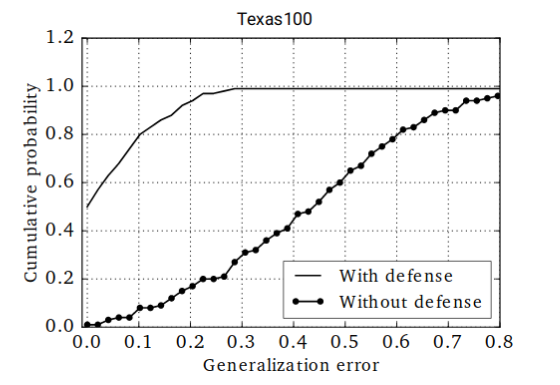
\includegraphics[width=2in]{regularization.png}
  \end{figure}
\end{frame}

\begin{frame}{Provable Method: Training with Differential Privacy}
  \begin{itemize}[<+-| alert@+>]
    \item \emph{Differential Privacy} is a property of a probabilistic training procedure $T(X)$.
      For any $X$, $X'$ differing by a single example, corresponding classifiers $\theta = T(X)$,
      $\theta' = T(X')$ are $\varepsilon$-similar.
    \item Formally, for any two datasets $X$, $X'$ differing by one example:
      \[
        D(T(X) \parallel T(X') ) \leq \varepsilon,
      \]
      where $D$ is distance between distributions. Usually $\infty$-R\'enyi.
      % \[
      %   \sup_{\theta} \log \sup_{\theta} \frac{\Pr[T(X) = \theta]}{\Pr[T(X') = \theta'] \right}
      % \leq \varepsilon
     % \]
    \item For example, clipping and randomizing gradient updates in gradient descent results in some
      differential privacy:
      \[
        \theta := \textsf{Clip} \left[ \theta + \alpha \nabla L(x, y; \theta) + \textsf{noise}\right]
      \]
    \item The lower $\varepsilon$ the higher privacy.
    \item There are efficient differential private training procedures that work well with
      $\varepsilon = 0.1$ (\cite{IyengarNSTTW19}). For comparison, Apple uses $\varepsilon = 15$).
  \end{itemize}
\end{frame}

\begin{frame}{Takeaways}
  \begin{itemize}[<+-| alert@+>]
    \item ML models leak the data left and right: they overfit and memorize
    \item Adversaries can often infer if the data points were present in the training data, and
      learn unknown parts of these data points
    \item As with adversarial robustness, solving this issue could benefit both generalization
      performance and privacy
    \item Unlike other problems in security, there exist cryptographically strong defences
      (differential privacy), that you should use wherever possible.
  \end{itemize}
\end{frame}


\section{Privacy and Security against Machine Learning}

\begin{frame}{Pitfalls of High Costs of Errors}
  \begin{itemize}[<+-| alert@+>]
    \item Threats from adversaries
    \item ML often finds correlation, not causation
    \item Societal biases learned from data
    \item Produce errors due to distributional shift
    \item Base-rate fallacy. Need extremely high recall in highly class-unbalanced problems
    \item Reward hacking: get good score without fulfilling the purpose
    \item Distribute errors unfairly
    \item In general: result in antisocial and negative \emph{environmental} outcomes
  \end{itemize}
\end{frame}

\begin{frame}{Example: Accidental Disparate Impact}
  \begin{figure}
    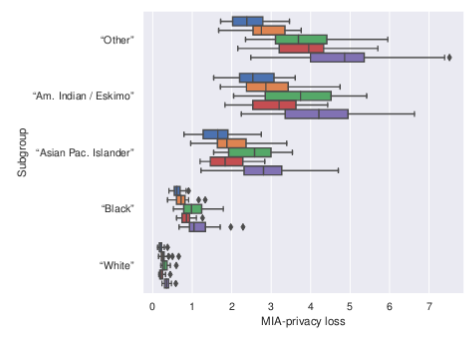
\includegraphics[width=3in]{losses.png} \\
    Image Credit: Yaghini et al. 2019
  \end{figure}
\end{frame}

\begin{frame}{Illegitimate uses: Manipulation}
  \begin{figure}
    \centering
    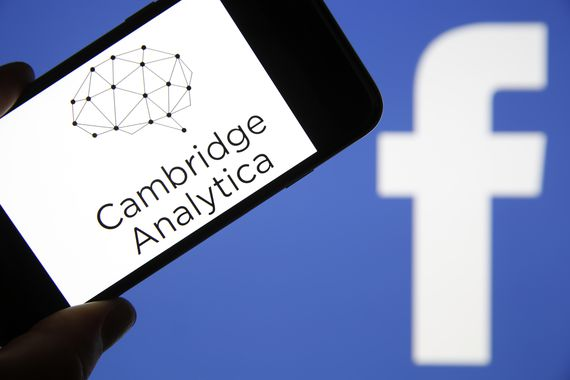
\includegraphics[width=3in]{cambridge_analytica.jpg} \\
  \end{figure}
\end{frame}

\begin{frame}{Illegitimate uses: Private Attribute Inference}
  \begin{figure}
    \centering
    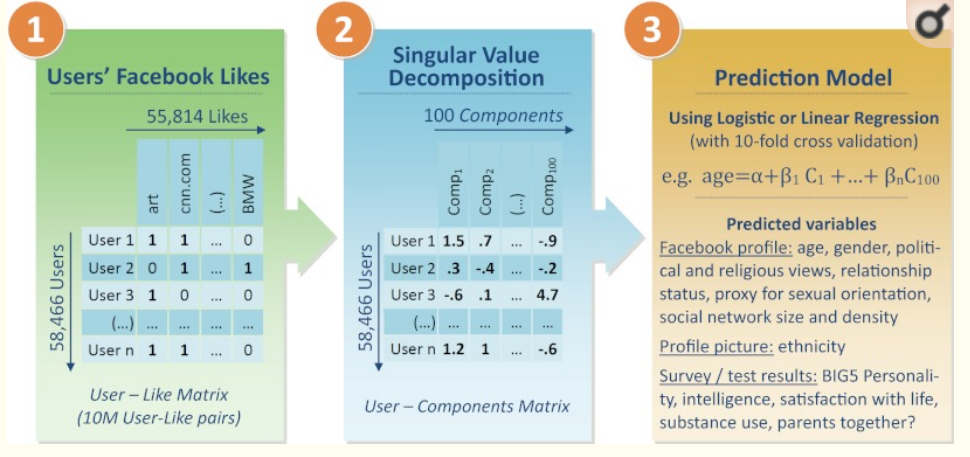
\includegraphics[width=3in]{likes.png} \\
    Image Credit: Kosinski et al. 2019
  \end{figure}
\end{frame}

\begin{frame}{Open Problems}
  \begin{itemize}[<+-| alert@+>]
    \item How do we protect people against these?
    \item We can use adversarial ML attacks \emph{as defences} (\cite{OverdorfKBTG18})
    \item These threat models are not considered at all
    \item Context and impact of models matters
  \end{itemize}
\end{frame}

% \appendix

% \begin{frame}[fragile]{Backup slides}
% \end{frame}

\begin{frame}[allowframebreaks]{References}

  \bibliography{main}
  \bibliographystyle{unsrtnat}

\end{frame}

\end{document}
